\section{Introduction}
\label{sec:introduction}

Vision-language-action (VLA) models map visual observations and language instructions to robot actions~\cite{brohan2023rt2,octo2024,kim2024openvla,black2024pi0,intelligence2025pi05,bjorck2025groot}. Their multimodal backbones and iterative action generators make model storage a practical deployment constraint. Post-training quantization (PTQ) reduces this footprint without retraining~\cite{xiao2023smoothquant,lin2024duquant}. For a robot, however, the useful outcome is a compact policy that still completes its tasks. A small reconstruction error on calibration tensors is an intermediate criterion, not that deployment objective.

Closed-loop control makes this distinction consequential. A quantized action can change the next observation, which changes the activations and errors encountered by the policy thereafter. Calibration on a fixed teacher buffer does not directly evaluate this policy-dependent input distribution. The practical discrepancy can be large: on 50 RoboCasa365 tasks, two GR00T configurations with approximately 0.90~GiB of static storage obtain 30.4\% success for QuantVLA and 54.0\% for our deployment, compared with 55.1\% for the larger FP16 reference. Similar storage therefore does not imply similar behavior. This motivates our central question: \emph{how should VLA quantization account for the behavior and inputs induced by the compressed policy?}

We study this question through complete-policy deviation and deployment-conditioned activation ranges. Ordered action errors expose accumulated bias and replanning discontinuities that isolated tensor errors omit; complete precision configurations expose interactions that additive layer scores approximate; and input-conditioned ranges avoid relying exclusively on frozen calibration coverage. We refer to the missing dependence on execution context as the \emph{full-context gap}. Closed-loop error propagation itself is not new, and these considerations do not amount to solving the induced-distribution problem. Our contribution is to connect them to concrete VLA quantization choices and test their behavioral consequences with matched interventions.

We introduce \method, a training-free framework with an offline precision stage and an input-conditioned deployment stage. Offline, a representation-stability allocator supplies an initial mixed W4/FP16 mask. Full-Context Precision Protection (FCP) evaluates complete-policy interventions to fit a transferred mask within an exact byte ceiling and admits later refinements only under predeclared deviation guards. At deployment, a standard per-forward, per-channel max-abs rule computes 8-bit activation ranges from the actual input. The precision mask stays fixed: the policy neither routes by task nor applies output correction. The method combines established quantization primitives with an explicit behavioral audit; the evidence for each component is evaluated separately.

\begin{figure}[t]
  \centering
  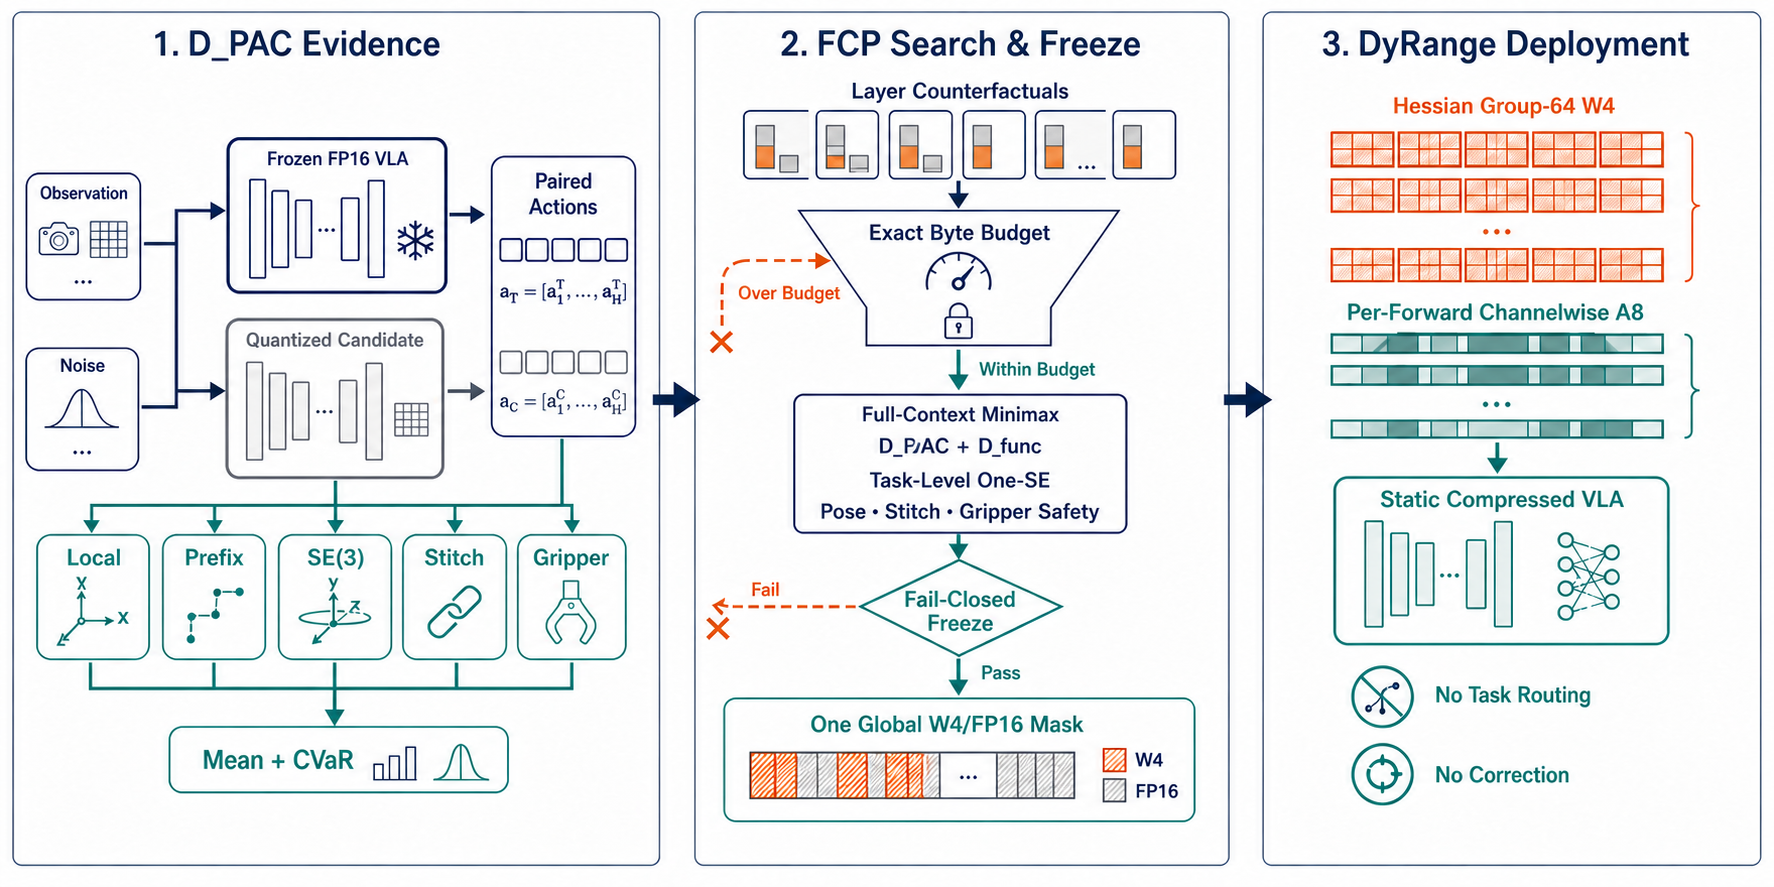
\includegraphics[width=\textwidth]{figures/dypac_main_architecture_api_v2.png}
  \caption{Overview of \method. Paired physical action chunks produce \dpac evidence; \fcp filters exact-budget masks with full-context, task-level upper bounds and freezes one global W4/FP16 plan; deployment combines Hessian group-64 W4 with per-forward \dyrange, without task routing or output correction.}
  \label{fig:pipeline}
\end{figure}


The results distinguish system effectiveness from component necessity. GR00T achieves 54.0\% success at 2.22$\times$ static compression, a 23.6-point improvement over size-matched QuantVLA. A fixed-mask intervention changes only activation-range construction and yields 269/500 successes with input-conditioned A8 versus 0/500 for the registered frozen table. On $\pi_{0.5}$, the precision stage converts an over-budget initializer into a feasible policy with 27.7\% success at 2.70$\times$ compression; FP16 obtains 26.2\%. The latter difference is descriptive, rather than evidence that quantization generally improves policy capability. A six-arm GR00T sweep is non-monotonic in FP16 layer count, and the GR00T audit retains its initializer. These outcomes delimit what the framework establishes, while a 4,000-episode LIBERO matrix tests cross-benchmark transfer.

Our contributions are threefold.
\begin{enumerate}[label=(\arabic*)]
    \item \textbf{Closed-loop quantization analysis.} We formulate compression as task success under an exact storage budget and distinguish local reconstruction, complete-policy deviation, and realized-input range construction. Matched interventions test the consequences of deployment choices rather than assuming that offline fidelity predicts success.
    \item \textbf{Budgeted adaptation and input-conditioned deployment.} We combine a guarded initializer with complete-policy precision adaptation and standard dynamic A8. On $\pi_{0.5}$, adaptation removes 41 FP16 protections to meet the target budget; on GR00T, the audit retains the feasible initializer without establishing its optimality.
    \item \textbf{Success--storage evidence and boundaries.} We evaluate two architectures on RoboCasa365 and LIBERO, isolate post-allocation effects, and report compression sweeps and rejected candidates. The results support competitive compressed policies while exposing limits of proxy ranking, mixed-precision necessity, and runtime efficiency.
\end{enumerate}